صفحه را به موزاییک‌های $3\times1$ بدون در نظر گرفتن یک خانه‌ای که اضافه می‌آید، تقسیم می‌کنیم. 
	\p
\begin{center}
    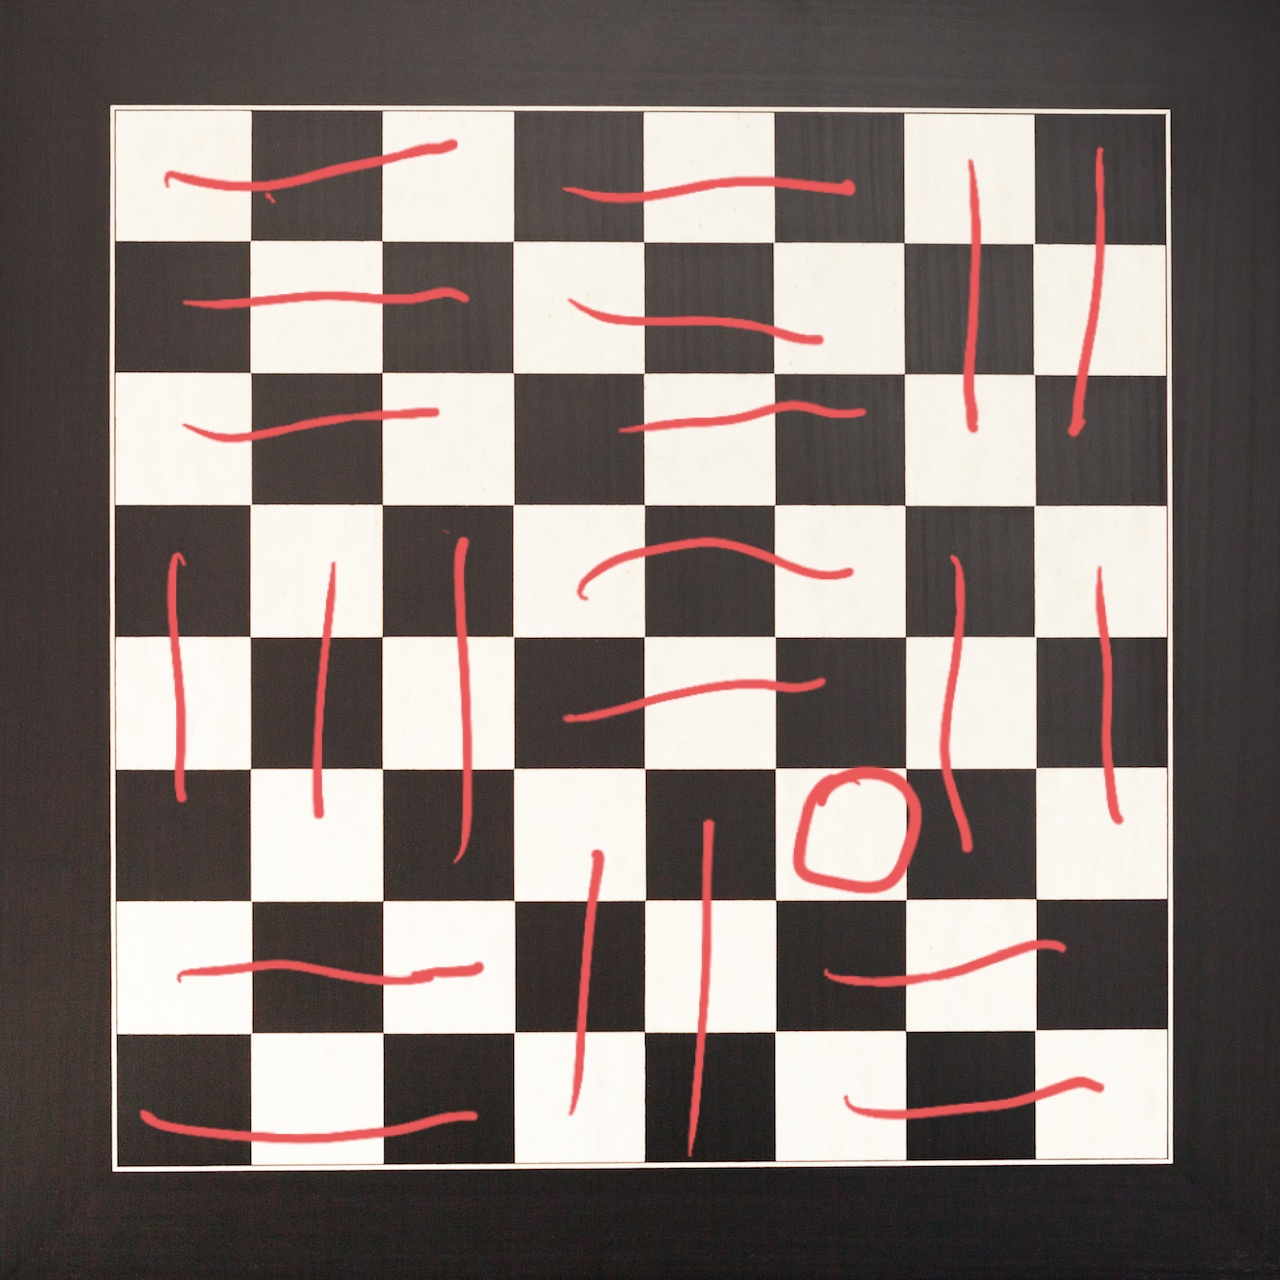
\includegraphics[height=5cm]{Q3Pic.jpg}
\end{center}
(خانه اضافه با توجه به نحوه چینش‌، در جاهای مختلف صفحه می‌تواند قرار بگیرد. به طور مثال در شکل، خانه اضافه در سطر و ستون ششم واقع شده است.)
	\p
 در حالتی که آن خانه بنفش باشد، طبق اصل لانه کبوتری در
$21$ 
موزاییک ایجاد شده حداقل
$43$
خانه رنگ شده وجود دارد، پس بر اساس اصل لانه کبوتری حداقل 
$1$
موزاییک وجود دارد که هر 
$3$ 
خانه‌اش رنگ شده باشد.
\[[\frac {43} {21}]+1=3\]  
در حالتی که خانه اضافه بنفش نباشد، هم می‌توان به همین شکل اثبات کرد.
\[[\frac {44} {21}]+1=3\]  